\documentclass[11pt,twoside,a4paper]{article}
\usepackage{tikz}

\usepackage{bera}% optional: just to have a nice mono-spaced font
\usepackage{listings}
\usepackage{xcolor}

\colorlet{punct}{red!60!black}
\definecolor{background}{HTML}{EEEEEE}
\definecolor{delim}{RGB}{20,105,176}
\colorlet{numb}{magenta!60!black}

\lstdefinelanguage{json}{
    basicstyle=\normalfont\ttfamily,
%    numbers=left,
%    numberstyle=\scriptsize,
%    stepnumber=1,
%    numbersep=8pt,
%    showstringspaces=false,
%    breaklines=true,
%    frame=lines,
%    backgroundcolor=\color{background},
%    literate=
%     *{0}{{{\color{numb}0}}}{1}
%      {1}{{{\color{numb}1}}}{1}
%      {2}{{{\color{numb}2}}}{1}
%      {3}{{{\color{numb}3}}}{1}
%      {4}{{{\color{numb}4}}}{1}
%      {5}{{{\color{numb}5}}}{1}
%      {6}{{{\color{numb}6}}}{1}
%      {7}{{{\color{numb}7}}}{1}
%      {8}{{{\color{numb}8}}}{1}
%      {9}{{{\color{numb}9}}}{1}
%      {:}{{{\color{punct}{:}}}}{1}
%      {,}{{{\color{punct}{,}}}}{1}
%      {\{}{{{\color{delim}{\{}}}}{1}
%      {\}}{{{\color{delim}{\}}}}}{1}
%      {[}{{{\color{delim}{[}}}}{1}
%      {]}{{{\color{delim}{]}}}}{1},
}
\lstset{language=json}

\begin{document}
\title{{\em Ledger Loops}: Hashlocked IOUs make the world go round.}
\author{Michiel B. de Jong}
\date{September 2018}
\maketitle
\begin{abstract}
LedgerLoops is a novel financial technology. Ra\-ther than a cryp\-to-cur\-ren\-cy or new form of mo\-ney, it is better viewed as an alternative to money. At its core is the concept of {\em hashlocks}.

In this whitepaper, the Whispering Merchants problem serves as a simplified abstraction of economic exchange in general, where assets flow in loops. Traditionally, money would flow in the opposite direction, thus solving the coordination problem by effectively reducing the loop to a chain of one-to-one transactions. But money has a number of downsides, mainly due to the need to trust people other than your direct economical neighbors. Value fluctuations in a currency act as a single point of failure, which can have devastating effects on economic trade. LedgerLoops aims to allow assets to move around, while every trader only needs to trusts their own direct peers.

LedgerLoops is a novel solution to the Whispering Merchants problem, based on a cryptographic trigger (hashlock) which activates each local IOU, ra\-ther than mo\-ving some sort of currency around the circle of merchants in the opposite direction.
\end{abstract}

\section{The Whispering Merchants Problem}
In the Whispering Merchants problem, merchants sit in a circle, facing outward. Each merchant can only communicate with their two direct neighbors in the circle. Each merchant wants to offer an asset to their clockwise neighbor, and obtain an asset from anti-clockwise neighbor. Each merchant trusts their immediate neighbors to keep any promises they make, but they do not trust anyone else (thus excluding fiat money as an option), nor are they interested in any other asset than the item offered by their anti-clockwise neighbor (thus excluding commodity money). The problem exists in achieving cooperation between the merchants so that all assets move clockwise by one merchant.

To give an example, consider 4 merchants, Abraham, Bethany, Chad and Dorus, sitting in a circle, facing outward.

\begin{figure}
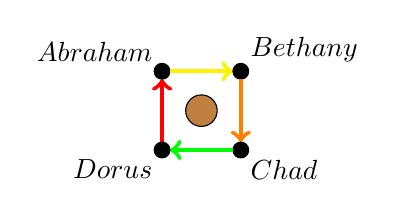
\begin{tikzpicture}
\draw [fill=brown] (0.5, 0.5) circle [radius=0.2];

\draw[->,red,ultra thick] (0,0.1) --(0,0.9);
\draw [fill=black] (0,1) circle [radius=0.1];
\node[above left] at (0,1) {$Abraham$};

\draw[->,yellow,ultra thick] (0.1,1) --(0.9,1);
\draw [fill=black] (1, 1) circle [radius=0.1];
\node[above right] at (1,1) {$Bethany$};

\draw[->,orange,ultra thick] (1,0.9) --(1,0.1);
\draw [fill=black] (1,0) circle [radius=0.1];
\node[below right] at (1,0) {$Chad$};

\draw[->,green,ultra thick] (0.9,0) --(0.1,0);
\draw [fill=black] (0, 0) circle [radius=0.1];
\node[below left] at (0,0) {$Dorus$};
\end{tikzpicture}
\caption{Abraham has a \textbf{\color{yellow} Banana} to offer Bethany. Bethany has a \textbf{\color{orange} Carrot} for Chad. Chad has a \textbf{\color{green} Durian} for Dorus. Dorus, in turn, has an \textbf{\color{red} Apple} to offer, in which Abraham is interested.}
\end{figure}

\begin{figure}
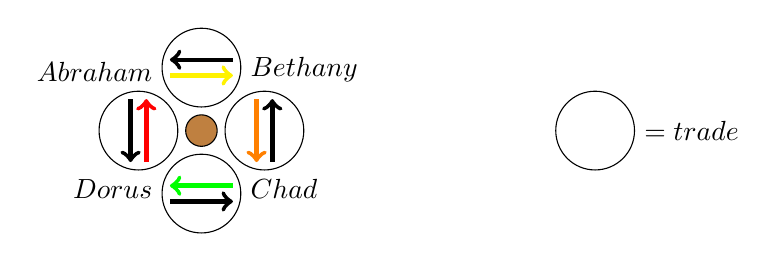
\begin{tikzpicture}
Abraham: 0,1
Bethany: 0,0 -> 1,1
Chad: 1,0
Dorus: 1,1 -> 0,0

\draw [black] (1.3, 0.5) circle [radius=0.5];
\draw [black] (0.5, 1.3) circle [radius=0.5];
\draw [black] (0.5, -0.3) circle [radius=0.5];
\draw [black] (-0.3, 0.5) circle [radius=0.5];

\draw [black] (5.5, 0.5) circle [radius=0.5];
\node[right] at (6.0, 0.5) {$= trade$};

\draw [fill=brown] (0.5, 0.5) circle [radius=0.2];

\draw[->,red,ultra thick] (-0.2,0.1) --(-0.2,0.9);
\draw[<-,black,ultra thick] (-0.4,0.1) --(-0.4,0.9);
\node[above left] at (0,1) {$Abraham$};

\draw[->,yellow,ultra thick] (0.1,1.2) --(0.9,1.2);
\draw[<-,black,ultra thick] (0.1,1.4) --(0.9,1.4);
\node[above right] at (1,1) {$Bethany$};

\draw[->,orange,ultra thick] (1.2,0.9) --(1.2,0.1);
\draw[<-,black,ultra thick] (1.4,0.9) --(1.4,0.1);
\node[below right] at (1,0) {$Chad$};

\draw[->,green,ultra thick] (0.9,-0.2) --(0.1,-0.2);
\draw[<-,black,ultra thick] (0.9,-0.4) --(0.1,-0.4);
\node[below left] at (0,0) {$Dorus$};
\end{tikzpicture}
\caption{Using money to decompose the flow of assets, into four one-on-one transactions. Money is the traditional standard solution for clearing trade between strangers, and requires a monetary token to travel in the counter-direction of the trade flow (black arrows). Each participant takes a devaluation risk from the moment they accept the token to the moment they successfully forward it.}
\end{figure}

\begin{figure}
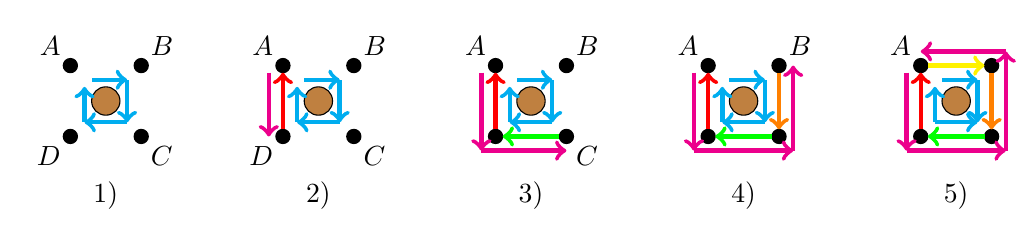
\begin{tikzpicture}[scale=0.9]
% letters
\node[above left] at (0,1) {$A$};
\node[above left] at (3,1) {$A$};
\node[above left] at (6,1) {$A$};
\node[above left] at (9,1) {$A$};
\node[above left] at (12,1) {$A$};

\node[above right] at (1,1) {$B$};
\node[above right] at (4,1) {$B$};
\node[above right] at (7,1) {$B$};
\node[above right] at (10,1) {$B$};

\node[below right] at (1,0) {$C$};
\node[below right] at (4,0) {$C$};
\node[below right] at (7,0) {$C$};

\node[below left] at (0,0) {$D$};
\node[below left] at (3,0) {$D$};

% numbers
\node[below] at (0.5,-0.5) {$1)$};
\node[below] at (3.5,-0.5) {$2)$};
\node[below] at (6.5,-0.5) {$3)$};
\node[below] at (9.5,-0.5) {$4)$};
\node[below] at (12.5,-0.5) {$5)$};

% trees
\draw [fill=brown] (0.5, 0.5) circle [radius=0.2];
\draw [fill=brown] (3.5, 0.5) circle [radius=0.2];
\draw [fill=brown] (6.5, 0.5) circle [radius=0.2];
\draw [fill=brown] (9.5, 0.5) circle [radius=0.2];
\draw [fill=brown] (12.5, 0.5) circle [radius=0.2];

% step 1 cyan and black
\draw[<-,cyan,ultra thick] (0.8,0.8) --(0.3,0.8);
\draw [fill=black] (0,1) circle [radius=0.1];

\draw[<-,cyan,ultra thick] (0.8,0.2) --(0.8,0.8);
\draw [fill=black] (1,1) circle [radius=0.1];

\draw[<-,cyan,ultra thick] (0.2,0.2) --(0.8,0.2);
\draw [fill=black] (1,0) circle [radius=0.1];

\draw[<-,cyan,ultra thick] (0.2,0.7) --(0.2,0.2);
\draw [fill=black] (0,0) circle [radius=0.1];

% step 2 cyan and black
\draw[<-,cyan,ultra thick] (3.8,0.8) --(3.3,0.8);
\draw [fill=black] (3,1) circle [radius=0.1];

\draw[<-,cyan,ultra thick] (3.8,0.2) --(3.8,0.8);
\draw [fill=black] (4,1) circle [radius=0.1];

\draw[<-,cyan,ultra thick] (3.2,0.2) --(3.8,0.2);
\draw [fill=black] (4,0) circle [radius=0.1];

\draw[<-,cyan,ultra thick] (3.2,0.7) --(3.2,0.2);
\draw [fill=black] (3,0) circle [radius=0.1];

% step 3 cyan and black
\draw[<-,cyan,ultra thick] (6.8,0.8) --(6.3,0.8);
\draw [fill=black] (6,1) circle [radius=0.1];

\draw[<-,cyan,ultra thick] (6.8,0.2) --(6.8,0.8);
\draw [fill=black] (7,1) circle [radius=0.1];

\draw[<-,cyan,ultra thick] (6.2,0.2) --(6.8,0.2);
\draw [fill=black] (7,0) circle [radius=0.1];

\draw[<-,cyan,ultra thick] (6.2,0.7) --(6.2,0.2);
\draw [fill=black] (6,0) circle [radius=0.1];

% step 4 cyan and black
\draw[<-,cyan,ultra thick] (9.8,0.8) --(9.3,0.8);
\draw [fill=black] (9,1) circle [radius=0.1];

\draw[<-,cyan,ultra thick] (9.8,0.2) --(9.8,0.8);
\draw [fill=black] (10,1) circle [radius=0.1];

\draw[<-,cyan,ultra thick] (9.2,0.2) --(9.8,0.2);
\draw [fill=black] (10,0) circle [radius=0.1];

\draw[<-,cyan,ultra thick] (9.2,0.7) --(9.2,0.2);
\draw [fill=black] (9,0) circle [radius=0.1];

% step 5 cyan and black
\draw[<-,cyan,ultra thick] (12.2,0.7) --(12.2,0.2);
\draw [fill=black] (12,0) circle [radius=0.1];

\draw[->,cyan,ultra thick] (12.2,0.2) --(12.8,0.2);
\draw [fill=black] (13,0) circle [radius=0.1];

\draw[<-,cyan,ultra thick] (12.8,0.2) --(12.8,0.8);
\draw [fill=black] (13,1) circle [radius=0.1];

\draw[<-,cyan,ultra thick] (12.8,0.8) --(12.3,0.8);
\draw [fill=black] (12,1) circle [radius=0.1];

% red and its magenta:
\draw[->,magenta,ultra thick] (2.8,0.9) --(2.8,0); % 0 instead of -0.2 to avoid hitting the D
\draw[<-,red,ultra thick] (3,0.9) --(3,0.1);
\draw[->,magenta,ultra thick] (5.8,0.9) --(5.8,-0.2);
\draw[<-,red,ultra thick] (6,0.9) --(6,0.1);
\draw[->,magenta,ultra thick] (8.8,0.9) --(8.8,-0.2);
\draw[<-,red,ultra thick] (9,0.9) --(9,0.1);
\draw[->,magenta,ultra thick] (11.8,0.9) --(11.8,-0.2);
\draw[<-,red,ultra thick] (12,0.9) --(12,0.1);

% green and its magenta:
\draw[->,magenta,ultra thick] (5.8,-0.2) --(7.0,-0.2); % 7.0 instead of 7.2 to avoid hitting the C
\draw[<-,green,ultra thick] (6.1,0) --(6.9,0);
\draw[->,magenta,ultra thick] (8.8,-0.2) --(10.2,-0.2);
\draw[<-,green,ultra thick] (9.1,0) --(9.9,0);
\draw[->,magenta,ultra thick] (11.8,-0.2) --(13.2,-0.2);
\draw[<-,green,ultra thick] (12.1,0) --(12.9,0);

% orange and its magenta:
\draw[->,magenta,ultra thick] (10.2,-0.2) --(10.2,1.0); % 1.0 instead of 1.2 to avoid hitting the B
\draw[<-,orange,ultra thick] (10,0.1) --(10,0.9);
\draw[->,magenta,ultra thick] (13.2,-0.2) --(13.2,1.2);
\draw[<-,orange,ultra thick] (13,0.1) --(13,0.9);

% yellow and its magenta:
\draw[->,magenta,ultra thick] (13.2,1.2) --(12.0,1.2); % 12.0 instead of 11.8 to avoid hitting the A
\draw[<-,yellow,ultra thick] (12.9,1.0) --(12.1,1.0);
% 01 2 34 5 67 8 90 1 23

\end{tikzpicture}
\caption{Step 1) Each participant uses the same hashlock to send a \textbf{\color{cyan} cryptographically triggered IOU}. Step 2) Only Abraham can solve the hashlock, and uses the solution as a \textbf{\color{magenta} LedgerLoops trigger} to claim the {\color{red} Apple}. Step 3) Dorus reuses the trigger to claim the {\color{green} Durian}. Step 4) Chad can now claim the {\color{orange} Carrot}. Step 5) Bethany claims the {\color{yellow} Banana} from Abraham. This safely coordinates all four transactions in one atomic trigger.}
\end{figure}

What makes the Whispering Merchants problem hard is that for instance in this example, Abraham initially has no way of obtaining the apple from Dorus, since he has nothing of interest to offer to Dorus. Abraham also has no knowledge of the existence of Chad, and he does not trust Chad.

The LedgerLoops website (https://ledgerloops.com) contains a discussion of various money systems, none of which satisfy the requirement that each participants only trusts their own immediate neighbors.

\section{Hashlocks}
This whitepaper proposes a solution to the Whispering Merchants problem, called LedgerLoops. It is based on cryptographic triggers ('hashlocks').

A hashlock consists of two parts: a challenge and a solution. The challenge can be included as a condition in contracts. Once the solution has been made public, all contracts are activated.

An IOU (short for "I owe you") is a message or document representing a debt.
A hashlocked IOU contains the same data as a standard IOU (debtor, beneficiary, asset owed, etc.), plus a hashlock challenge.

The IOU is without value until the beneficiary presents a solution of the hashlock. In the current version of the LedgerLoops protocol, the hashlock challenge is defined by the SHA-256 hash of a random string; the challenge is simply to find the string (or more precisely, {\i a} string) that has the hash value from the challenge. Only the person holding the original string will be able to do this, yet everybody can easily verify and agree if a given candiate solution to the challenge is valid or not.

The Whispering Merchants can use hashlocked IOUs as follows to facilitate their trade. One merchant creates a hashlock by picking a 256-bit string at random (the solution, which they keep secret) and calculating its SHA-256 hash value (the challenge, which is included as the condition in hashlocked IOU contracts). The identity of this initiator stays obfuscated. Remember all merchants are willing to give their asset to their clockwise neighbor, but only if they can be sure that their own anti-clockwise neighbor will do the same.

The initiator gives a hashlocked IOU to his clockwise neighbor, for the item he wants to offer. Each next clockwise neighbor does the same. The details of the hashlock challenge are reused each time, but the item offered is different in each locally created IOU.

Once the initiator receives a hashlocked IOU from his own anti-clockwise neighbor, for the item he wants to receive, he presents the solution (now made public for the first time) to his anti-clockwise neighbor. Each next anti-clockwise neighbor now gives the asset they offered in exchange for the solution to the challenge.

Since the challenge used in all hashlocked IOUs was the same one for all trades along the loop, the solution to this challenge acts as a cryptographic trigger, but its meaning is different from the meaning of a cryptographic coin: it represents no value, it only represents a "Go!" signal which all participants recognize. Therefore, LedgerLoops should be considered an alternative to money, rather than an alternative form of money.

\section{The LedgerLoops Protocol (version 0.8)}
In 2016, I have implemented a few design iterations of the LedgerLoops protocol. Future versions are likely to differ from this, but let me describe roughly how the current version works.

\subsection{Peer-to-peer Ledgers}
As Graeber noted in his book "Debt: the first 5,000 years" ~\cite{Graeber2011}, peer-to-peer debt is useful for (in my words) time-skewed barter between two peers: I give you something now, and you give me something in exchange tomorrow; in the meantime, a debt exists. This is why LedgerLoops is based on peer-to-peer ledgers (that is, ledgers on which two people keep track of what they owe each other).

Before finding a loop along which assets can move around, the first step of the algorithm consists of agents building up a ledger with each of their neighbors in the graph, by sending each other standard, unconditional IOUs, of the following format:

\vbox{\begin{lstlisting}
{
  "protocol": "ledgerloops-0.8",
  "msgType": "ADD",
  "msgId": <integer>,
  "note": "<a description of why this entry is added>,
  "beneficiary": "<identifies party gaining balance; just a nickname>",
  "sender": "<usually the other party in the two-peer ledger; just nickname>",
  "amount": <integer>,
  "unit": "UCR"
}
\end{lstlisting}}

The Unicurn ("UNIversal CUrrency RefereNce" / "UCR") is defined relative to a trade-weighted basket of reference currencies, see https://unicurn.com (I'm still working on defining this).

Even if the communication network is reliable and would detect network outages without losing any messages, a malfunction in the receiver's software could make it look like this message was received successfully when in fact it was not, so to confirm receipt, the recipient replies with:

\vbox{\begin{lstlisting}
{
  "protocol": "ledgerloops-0.8",
  "msgType": "ACK",
  "sender": "<same as in ADD message>",
  "msgId": "<same as in ADD message>"
}
\end{lstlisting}}

As soon as the 'ACK' message has been sent, both peers update their copy of the ledger by appending this one entry.
So in the current implementation, LedgerLoops coordination is used to create or cancel debts, not directly to trigger the movement of assets. Each participant will be happy if they can exchange one of their incoming debts against one of their outgoing debt, since the balance of each debt will go down, thereby minimizing their exposure to credit risk and enabling new trades to take place. Also, peers can offer goods first, and only if a loop is found, commit to actually owing the delivery of these goods.

\subsection{Routing}

The Whispering Merchants problem is a best-case scenario for using LedgerLoops, since all merchants have exactly one in-neighbor (their anti-clockwise neighbor who offers an asset) and one out-neighbor (their clockwise neighbor, to whom they offer an asset). In a real economy, asset offers could form any directed graph between agents, and agents should first cooperate to detect if any cycles actually exist.

Finding cycles in a graph of which no one has a bird's eye view is an interesting computer science problem. Recently, 'Distributed Cycle Detection and Removal' ~\cite{Oliva2016} ('DCD') was included in a non-free IEEE publication. Unfortunately, due to the scientific journal's policy, no public version of the algorithm is available yet (you can buy the article from the IEEE website), but I can try to explain it in my own words:

\begin{itemize}
\item each leaf node (one that has either only in-neighbors or only out-neighbors), goes into 'deactivated' mode, and initiates a bread-first wave of messages through the network; from the point of view of each node, these messages mean as much as "I am sure I'm not part of a cycle".
\item each internal node will go into 'deactivated' mode and forward the wave of messages to their out-neighbors as soon as they have received a message from each of their in-neighbors. Vice versa, they will send out a message to all their in-neighbors as soon as they have received one from all their out-neighbors.
\item after waiting long enough, nodes that have not deactivated yet, can know that they are either on a cycle, or on a path from one cycle to another. At least, nodes that want to start a depth-first search for cycles, can now discard all neighbors from whom they receive such a message, and drastically reduce their search space.
\end{itemize}

This algorithm is more decentralized than Rocha-Thatte. Another simple algorithm would be to forward tokens from node to node, along a depth-first search ('DFS'), until a back-edge is found.

I previously worked on a combination of DCD with DFS, but I now think that DCD's "I am not part of a loop" messages are hard to use in a changing graph where cycles are created and removed often. Instead, I'm now just using BFS in both directions whenever an edge is added to the network: Bidirecional Breadth-First Search (BBFS).

\subsubsection{Bidirectional Breadth-First Search (BBFS)}
Consider a network of interconnected agents. Each agent can decide that they want to participate in a LedgerLoop, accepting a COND message from what we'll call their "C-side" neighbor, and forwarding it to what we will call their "F-side" neighbor. When the F-side neighbor sends a FULFILL message in response, they'll also send a FULFILL message to their own C-side neighbor.

In order to coordinate the formation of LedgerLoops, agents can send each other PROBES messages. Each probe messages has a list of F-wise probes, traveling in the direction in which FULFILL messages would travel, and C-wise probes that travel in the direction in which COND messages would travel.

Agents will generally be able to define a partial ordering on their list of neighbors, such that neighbor C comes before neighbor F in the list if the agent would like to participate in a LedgerLoops where that neighbor C acts as their C-side neighbor, and that neighbor F acts as their F-side neighbor.

An agent can create a probe from scratch, by generating a random 16-byte string, and sending it as a C-wise probe to F, and also as an F-wise probe to C.

The format for a PROBES message is as follows:
\vbox{\begin{lstlisting}
{
  "protocol": "ledgerloops-0.8",
  "msgType": "PROBES",
  "cwise": [ <64 bits in a lower-case hex string>* ],
  "fwise": [ <64 bits in a lower-case hex string>* ]
}
\end{lstlisting}}

When a PROBES message comes in from neighbor C, the agent should forward the C-wise probes to neighbor F.
Likewise, when a PROBES message comes in from neighbor F, the agent should forward the F-wise probes to neighbor C.
An exception to this is if the same probe was already sent to the same neighbor before.
In case of a C-wise probe, the agent can send a COND instead.
In case of an F-wise probe, the agent could send a COND back to the neighbor who sent the F-wise probe, although this may lead to duplication where one pair of probes would trigger two LedgerLoops. 
It's up to each agent to decide how long to wait before forwarding probes, and whether to forward each probe to each eligible neighbor at all. That way, each agent has some say in how much bandwidth and CPU time they spend on the sending of probes.

It might seem like a very unwise idea to potentially generate a flood of messages across the whole network in response to a single local interaction between peers, but in practice I think the number of messages necessary will be within reason. To find all triangles, two agents only have to communicate their own friends list. To find all squares, that would be their own lists of friends-of-friends, etcetera. Say each agent has 10 friends, then that means 20, 200, 2000, and 20,000 probes for triangles, squares, pentagons and hexagons, respectively. This means a
Imagine each link between two agents is configured to have an amount of traffic comparable to one Internet Radio station (say 160 kbps, that's 20 Kb per second, that's 1280 probes/second), so this would mean that when a change in the network leads to the creation of a hexagon, it would be detected within 15 seconds. This is a conservative estimate, since nodes don't have to communicate their list of friends when the partial ordering on them hasn't changed.

\subsection{Hashlocked IOUs}

The initiator generates a random string and calculates its SHA-256 hash value. It then sends the following message to an out-neighbor:

\vbox{\begin{lstlisting}
{
  "protocol": "ledgerloops-0.8",
  "msgType": "COND",
  "msgId": <integer>,
  "condition": <256 bits in a lower-case hex string>,
  "note": "<a description of why this entry is added>,
  "beneficiary": "<identifies party gaining balance; just a nickname>",
  "sender": "<usually the other party in the two-peer ledger; just nickname>",
  "amount": <integer>,
  "unit": "UCR"
}
\end{lstlisting}}

Note that a sender can offer parts of a specific asset, even if the asset is a physical item that cannot be split into parts.
For instance, I could send you 10 IOUs, each referring to the blue bicycle I showed you as the "unit", and each for an amount of 0.1.
It is important to use each hashlock only once, so that it is clear which IOU is being triggered, and this is also tracked
correctly in our peer-to-peer ledger afterwards. As soon as I owe you 10 times one tenth of the blue bicycle, you can claim the
entire bicycle. You could also claim the bicycle after I owe you only 8 tenths of it, after which you would owe me the equivalent
of 2 tenths of the blue bicycle. This requires a more long-term form of trust between us than one-off trades of entire assets or
fungeable assets. Another option would be to value the blue bicycle in terms of a more common unit of value (for instance a standard
government-issued currency, a crypto-currency, a rare metal, or kiloWatt-hours of energy). This could simplify our peer-to-peer ledger.
For the conditional promise I send you, it only matters that we agree on what the unit of value refers to, and unlike currencies which are
used as money, this unit of value does not need to have any meaning to anyone apart from the two peers who discuss it.

Each participant reuses the 'condition' part of the con\-di\-tio\-nal pro\-mise they receive, and creates their own outgoing hashlocked IOU. The amount and unit should be roughly the same, so that when the forwarded COND message loops around to the initiator, the value is still roughly the same and the initiator will decide to publish the hashlock's solution. See the section about "Multi-lateral netting at equilibrium" below for a more precise discussion of exchange rate setting.

For now, the Unicurn is the only unit of value allowed for value estimates in COND messages.

Once a conditional promise message reaches the initiator, describing the unit of value the initiator desires, and promising an amount which the initiator finds acceptable compared to the amount of asset he offered when starting the loop, trade becomes possible. The initiator confirms that the incoming conditional promise message uses the same challenge
details which he created, and the solution to the challenge is sent round in the opposite direction:

\vbox{\begin{lstlisting}
{
  "protocol": "ledgerloops-0.8",
  "msgType": "FULFILL",
  "sender": "<sender of COND message>",
  "msgId": "<same id as COND message>",
  "preimage": "<original random string in lowercase hex format>",
}
\end{lstlisting}}

The receiver of a FULFILL message converts the solution field from its hex string representation, calculates the SHA-256 hash value of the resulting raw bytes, and converts the hash value back to lowercase hex representation. If the result matches the hash value from the challenge, the solution has been verified to be correct. The receiver replies with the "ACK"
message format from earlier (using the msgId from the "FULFILL" message) to confirm to the sender that the solution has been accepted, and the receiver agrees with the resulting update of their peer-to-peer ledger. The receiver has now lost the asset from their own earlier conditional promise, but has gained knowledge of the solution to the challenge used in all conditional promise messages sent earlier. He uses the solution to create his own FULFILL message and claim the asset that was conditionally promised to him by his other neighbor in the loop. Once all nodes along the loop have done this, the trade is complete.

Just like an ADD message, FULFILL message should be responded to with an ACK message in order to commit the proposed new entry to the peer-to-peer ledger on both sides.

If a node decides it has been waiting for too long, it can request a revokation of the hashlocked IOU they sent earlier,
by sending this messages behind it:

\vbox{\begin{lstlisting}
{
  "protocol": "ledgerloops-0.8",
  "msgType": "PLEASE-FINALIZE",
  "sender": "<sender of the COND message and also of this message>",
  "msgId": "<same id as the COND message>"
}
\end{lstlisting}}

A node should probably wait a few milliseconds before forwarding a cryptographically triggered IOU, in case the IOU has been buffered in
a slow place for a while, and now has a "PLEASE-FINALIZE" message following directly behind it.

To reject a hashlocked IOU you received earlier, use this message:

\vbox{\begin{lstlisting}
{
  "protocol": "ledgerloops-0.8",
  "msgType": "REJECT",
  "sender": "<sender of the COND message>",
  "msgId": "<same id as the COND message>"
  "reason": "human-readable free text",
}
\end{lstlisting}}

The rejection will only be valid if it is sent by the recipient of the COND message in question.

A REJECT message can also be used to reject an ADD or FULFILL message. So the message flows are: (1) ADD-ACK, (2) ADD-REJECT, (3) COND-[PLEASE-FINALIZE]*-FULFILL-ACK, (4) COND-[PLEASE-FINALIZE]*-FULFILL-REJECT, (4) COND-[PLEASE-FINALIZE]*-REJECT. Messages can be repeated to guarantee eventual agreement over a ledger entry (a ledger entry is uniquely defined by its sender and msgId).

\section{Security Discussion}
\subsection{Assessment Scope}
\subsubsection{At the participant level}
A participant in the LedgerLoops protocol is a human person or legal organization (the "user") who uses a computer on which LedgerLoops software (the "app") runs. This computer is potentially also used for other purposes. The user supplies contact details about other users (the user's "neighbors") to the app. This list of neighbors (containing contact details as well as personal notes such as nick names and profile photos) is sensitive information.

Once the user creates ledgers with their neighbors, the information in these ledgers (current balance as well as transaction history, and personal notes added to each transaction, which are likely to reflect evidence of real-world events) is the second item of sensitive information.

Each ledger is also personal between the user and the neighbor involved in that particular ledger; information from one ledger should not be leaked to one of the other ledgers, or become known to one of the user's other neighbors in some other way.

When the app starts trying to route and resolve loops, this activity affects other software on the same computer, by using network, CPU and storage resources. The app should also not leak or damage sensitive information pertaining to other software on the same computer.

If incorrect information were to enter the user's ledgers, the user's real-world assets could be at risk.
In this case, as well as when the app sends low-quality messages to neighbors, the user's reputation with their neighbors (debtors and creditors), and possibly the user's public reputation. An example of a low-quality message could be one that is malformed, or one that represents incorrect or unfounded information, like when the app were to continuously bother neighbors with messages that convey a statement of intent, convincing the neighbors to invest effort, but never or rarely leading to a trade deal, thus wasting other participants' time.

When the app initiates a LedgerLoops challenge, and the private key is lost, this is not a problem, because the app can reply with reject message instead of a satisfy-condition message when the time comes. If any of the other participants lose the solution while forwarding it, it could ask their debtor to resend it (this is not currently implemented, but this all seems quite low-risk, since the solution does not have any monetary value).

However, if the initiator's private key is leaked, this would oblige the initiator to fulfill their conditional promise, even if they themselves don't receive the item they desired.

To summarize, the user would be negatively affected if:

\begin{itemize}
\item any of the following information is leaked, either to one of the user's other neighbors, or publicly:
  \begin{itemize}
  \item identity of the user's neighbors
  \item information contained in notes about the user's neighbors
  \item ledgers (current balance as well as transaction history)
  \item information contained in notes on the ledgers
  \item other information, unrelated to the app but present on the computer
  \item the private key for a challenge that has not been solved yet
  \end{itemize}
  
\item the app would make excessive use of any of the following computer resources:
  \begin{itemize}
  \item network bandwidth
  \item CPU resources
  \item storage resources
  \end{itemize}
  
\item the app's copy of the following information would be damaged (it may trigger real-world events, or be the only copy of this data):
  \begin{itemize}
  \item ledger balance and transaction history
  \item other information, unrelated to the app but present on the computer
  \end{itemize}
  
\item the app's incorrect or unreasonable behavior damages the user's reputation with:
  \begin{itemize}
  \item debtor neighbors
  \item creditor neighbors
  \item third parties or the general public
  \end{itemize}
\end{itemize}

\subsubsection{At the network region level}
Once a number of users rely on the network beyond their own neighbors to find and resolve ledger loops, these users would be negatively
affected if this network clogs up or breaks down, affecting participants who are not neighbors of the user, but who would be candidates
to participate in a ledger loop in which the user and their neighbors would also participate.

Even if the valid participants of the network are unaffected, an excess number of useless participants would make the valid participants hard to find.

Likewise, useless network traffic could slow down the processing of valid network traffic.

The network as a whole is decentralized, and several independent regions (connected components in the network graph) could exist.
Low-quality areas in the network will mostly affect users at a short network distance from the low-quality region. Therefore,
in terms of valuable assets, we should consider network regions, more than the global network as a whole. We can write these assets at
the network region level down as:

\begin{itemize}
\item average quality of participants at distance d from a user (d>=2)
\item average quality of messages received from a user's neighbor, but triggered by messages at distance d>=2.
\end{itemize}

\subsection{System Modeling}
As already defined a bit in the previous subsection, a user uses the app running on a computer. The app sends LedgerLoops messages, only to direct neighbors of the users, although these messages might cause ripple effects, triggering messages to other participants at distance d>=2.
The messages sent between neighboring users travel over a secure communication channel (the sending and receiving client software for this communication channel is not part of the app). Neighbors of a user can be divided into two categories: debtor (owes or offers something to the user), and creditors (to whom the user owes or offers something). Incentives for cooperation can be different for debtors than for creditors. For instance, if a creditor misbehaves, the user can block them (ignore messages from them) and tell the neighbor user in question through a side channel to change their app's behavior if they still want to access their credit. If the creditor does not comply, the user can confiscate their credit. However, if a debtor misbehaves, the user cannot so easily block their messages, as this would effectively allow the debtor to never pay back their debt - or at least not pay it back via LedgerLoops.

\subsection{Threats}
\subsubsection{The user's own computer and LedgerLoops app}
While the user's app is running on the computer, it needs to access all information and resources mentioned in the assessment scope above. Therefore, a malfunctioning app would put all these assets at risk. When the user's computer is running, even if the app is not, there is probably no way to protect against potential malware on the computer. Even if the app stores its data in encrypted format, the user would have to unlock this data when starting to use the app, and any passphrase or secret used to do this while starting up the app could be intercepted by such malware. The computer as a whole could, however, use disk encryption so that if an attacker gains physical access to the computer, but can not force the user to enter their passphrase, the data stored on the computer would be safe. In short, if the user's computer is compromised, the attacker could access the user's information, damage the user's reputation, damage the user's real-world assets, and the user's reputation. A malfunction (bug) in the app could also potentially put all of these assets at risk.

The following threat descriptions all assume the user's computer is clean and the app functions correctly.

\subsubsection{Social Engineering}
A user could be convinced by an attacker to add a neighbor with whom they don't have a real-world trust relationship. Adding a ma\-li\-cious deb\-tor could expose information about the user's creditors. For instance, if an attacker wants to know if the user frequents a certain restaurant, they could buy a meal voucher from that restaurant, and at the same time offer something attractive to the user. If the user accepts the offer from the attacker, then the next time the user eats at that restaurant, the user's app could cooperate with the restaurant's app and the attacker's app to find a loop. If such a loop is found, then the attacker knows that either the user just visited the restaurant, or the user owes something to a participant, (who owes something to a participant, who \ldots) owes something to the restaurant.

Adding a malicious creditor could likewise expose information about the user's debtors.

\subsubsection{Network Area Attacks}
Nobody except a user's own neighbors is allowed to send the user messages directly, so standard Spam and Denial-of-Service attacks will not work to degrade a user's LedgerLoops app (it might still work to affect the user's computer or the user's internet connection, of course).

However, apart from the attacker becoming a neighbor of the victim (which should be quite hard if the user is careful), the attacker could try to control many nodes in the network area surrounding the user (so nodes that are two or three hops away from the victim). This would allow the attacker to degrade the quality of the user's network area,
for instance by injecting a lot of useless messages (low-quality traffic), and by making nodes look attractive for cooperation but never reaching agreement.

\subsubsection{Traffic Analysis}
Even if all of the user's neighbors (and their computers and their apps) are clean, an attacker in the same network area as the user could obtain information about the user by analysing their own ledger loops. If the attacker has several two-hop connections with the user, they could potentially analyse the messages they receive, and send their own messages to test hypotheses, to gather metadata about the user. They will not be able to know which of the ledger loops the user took part in, and it could be that what they are modeling as the targeted user is in fact two or three different users, but by playing it smart, they could potentially create an ever more detailed model of the targeted user.

\subsubsection{Figure-8 Attacks}
An attacker could aim to control two or more participants in the same ledger loops. However, if a ledger loop goes through participants 0, 1, 2, \ldots, 9, 0 and the attacker controls nodes 3 and 7, we can write this as "0, 1, 2, (3/7), 4, 5, 6, (3/7), 8, 9, 0". This is equivalent to two separate ledger loops: "0, 1, 2, (3/7), 8, 9, 0" and "(3/7), 4, 5, 6, (3/7)", where the $3 \rightarrow 7$ traffic from the first loop cancels out the $7 \rightarrow 3$ traffic from the second one. A threat where the attacker controls two nodes in a ledger loop can therefore be analyzed as two separate attacks.

\subsubsection{Timing Analysis}
One of the most worrisome threats may be timing analysis: in principle, a participant in a ledger loop knows that the ledger loop contains at least three participants, but does not know an upper bound of the number of participants. However, knowledge about network link speeds can help reveal such an upper bound. For instance, if the attacker knows that each network hops takes one second, and that a message was passed around the loop in four seconds, then they know there are no more than four participants in the loop. It does not work in the other direction: if a message takes 1000 seconds to go around the loop, this might be because one of the participants stalled for 996 seconds before forwarding the message. However, if all participants are known to always stall one second, then a roundtrip time of 8 seconds can also give evidence of a length-four loop. Randomizing the stall time helps a little bit to obfuscate loop length, but the attacker can average out this randomization by analyzing a large number of ledger loops together. Also, if all participants happen to randomly pick a low stall time, then a message could still travel around that loop in under 5 seconds. The most dangerous form of this threat is that where the attacker discovers with reasonable certainty that they are participating in a length-three loop, since this tells the attacker that their own debtor is also a neighbor of their own creditor.

\subsubsection{Lying}
LedgerLoops is a tool with which a user keeps track of debts and credit between themselves and their direct neighbors. The app has no leverage on the real world, other than through the user's own actions. This is why the neighbor always relies on the real-world trustworthiness of their own neighbors. For instance, an attacker who owes the user a significant asset could simply tell the user that their computer was compromised, and they no longer have a record of this debt. Even if the communication channel used cryptographic signatures, the attacker could deny having signed that message, stating that in fact some malware on their computer must have caused this message to be sent.

\subsection{Mitigation}
To mitigate the threats described above, a user should make sure their computer is clean, and use a peer-reviewed LedgerLoops app.
They should regularly make backups of ledger data, and regularly check if all ledgers still look as expected.
The app should help the use to block neighbors who send low-quality messages, and to contact them through other channels, resolving the issue before removing the block.
Users should not rely on their LedgerLoops app as the only record of their credits and debts, so that users can fall back on other records (emails, chat logs, paper documents etc.) in case a the information in a ledger becomes incorrect. Also, settling peer-to-peer debts before they become to big (for instance using plain-old-banking-system bank transfers) can help to keep the credit risk to which a user is exposed within reasonable limits.

\section{Roadmap}
The current version of the LedgerLoops protocol still lacks a few features. 

A LedgerLoops app could allow the user to define minimal exchange rates for pairs of assets the neighbor owes and is owed. The danger in this is that every candidate participant in a loop would try to make a profit, and the asset which the initiator is offered by their anti-clockwise neighbor would be worth much less than the asset the initiator offered for trade in the beginning. This brings the candidate participants into a sort of prisoner's dilemma: they should all try to make reasonable trade offers, otherwise no agreement will be reached, and nobody can trade. On the other hand, when agreement is reached, each participant could feel like they might have been able to negotiate a better deal if they would have negotiated a bit harder. This is a reality in all economic trade, but allowing it to occur in LedgerLoops negotiations will probably require more messages to be passed before a participants agree on a loop, and these extra messages may expose more information about each participant than in the current version of the protocol.

Finally, the current version of the protocol is limited to each participant trading part of one of their credits against part of one of their debts. In practice, it may be attractive for a user to exchange a partial reduction of debt at one creditor against an increase of debt at another creditor, or to exchange an increase of credit at one debtor for a decrease of credit at another debtor. This would require a change in the routing algorithm, since this makes every debtor and every creditor both a potential in-neighbor and a potential out-neighbor. The app would then probably allow users to indicate in more detail which creditors and which debtors they prefer over others (for instance, a user would typically prefer to have a credit at a neighbor they trust more, or with whom they have closer or more frequent real-world contact).

An advantage of this would be that users can choose to increase the general liquidity of their network surroundings by defining capacitances - for instance, instruct the app to always participate in a ledger loop in either direction with their closest friends for up to a set maximum of for instance 10 USD. If a close-nit group of friends all set a 10 USD capacitance with all their neighbors, this means more trades between one group member, and outsider, and another group member, become routable. Likewise, local hubs (like for instance a neighborhood community center, a bar, a sportsclub, or another place where people socialize) could act as capacitors, providing liquidity for users who often visit this place and have a ledger between themselves and the hub. Users could use a credit at the hub to pay for their drinks at the bar there, or in the case of a sports club, to pay their membership fee. Mobile phone operators who provide prepaid SIM cards could also act as capacitors, since the prepaid SIM card is essentially already a ledger (this is part of the reason behind the success of M-Pesa in Kenya).

The term capacitor / capacitance here comes from the analogy with the role these terms play in analysis of AC currents in analogue electronic circuits.

\section{Usability Discussion}
\subsection{Comparison with other financial technologies}
LedgerLoops has an obvious downside when compared to for instance crypto-currencies: a ledger update has no real-world effect unless you trust your own neighbors. You can only obtain credit in a LedgerLoops network if you have neighbors who you trust to keep this credit safe for you. Crypto-currencies don't perform very well either as a long-term value store, but at least they allow you to store your value against "the network in general", instead of having to pick a specific other participant.

However, given that users will supposedly have to trust their direct trade peers anyway, and as long as the user defines a maximum credit/debt level for which it trusts each neighbor, it also has obvious advantages over other currently known financial technologies.

Without the use of LedgerLoops, trade can only be facilited, and value can only flow around the economy, if it is offset by a counter-flow of some sort. This could be either a commodity that has real value, or some sort of token whose value is based on trust that your future trade peers will also attribute value to this sort of token.

Such trust in a (by itself worthless) token is often based on hype (hoping a certain crypto-currency will stay popular), or on war (politicians will generally send their soldiers to war to defend a government-issued currency when the power of the government is at risk), or on citizen-paid taxes (often used to bail out failing banks). LedgerLoops avoids this reliance on globally defined tokens, which makes it a much more decentralized technology. Any group of people can start to use the LedgerLoops protocol within their community, without relying on the health of a globally defined currency or on the health of a global network. If a hype of activity in LedgerLoops transaction rises and falls in some local geographic area, this has very little effect on the ability of people in another geographic area to use the LedgerLoops protocol. That being said, of course, communities would benefit from connecting with another community, and this would automatically happen if a few users form part of both communities. This network effect is very similar to how the internet works ("Connectivity is its own Reward").

\subsection{Starting to use LedgerLoops}
First of all, let me state that version 0.8 of LedgerLoops should be considered a developer preview, and further development will most likely be needed before the protocol is production-ready. Until we gain a better understanding of the network dynamics in more complex topologies, its use is only recommended for academic experiments, not for real-world trade. Users are advised to only trade very small assets, for instance up to 1 USD, since we can't yet predict what dynamics would arise, and what other security considerations may be discovered during such initial experiments.

Also, the current version of the software used on the demo page is not recommended for production; I probably need to rewrite it from scratch, using what I learned in the last few weeks developing this version 0.8 of LedgerLoops. Importantly, the code has also not been reviewed by a security expert yet, so it's not unlikely that this implementation contains a few vulnerabilities; in short, please only use it to run simulations, don't entrust it with data about your real-world trade peers yet.

One path to start using LedgerLoops in the real world, would be to develop an Android app which can access a smartphone's addressbook, and use the API of an existing end-to-end encrypted messaging platform for delivering the LedgerLoops messages to the user's neighbors. This would require a potential user to convince their real-world trade peers to install the same app, which would be impractical for casual one-time trade peers, but could work well for, for instance, people who share a house, or for the members of a sports club (where the administration of membership fees could be a driving use case).

Another path would be integration in existing peer-to-peer ledger apps, like Splitwise, Settle Up, and (to a lesser extent) payment and banking apps like the Dutch Bunq app and the German Opentabs.de app. Integration with LedgerLoops could be an interesting option for the publishers of such apps, as it could allow them to offer their existing users an attractive new feature: the ability to sometimes (not always) settle bills without requiring the user to register their creditcard or link their traditional bank account. Of course, if no LedgerLoop exists, none will be found, and the bill will stay unsettled as it is.

In any case, integrating the current version of the LedgerLoops protocol in an existing app is not yet recommended, but it could become an interesting innovation opportunity in the near future, once LedgerLoops grows out of the experimentation phase.

\section{Conclusion}
This is a work in progress, I hope you enjoyed reading it. Your comments and contributions would be very welcome, please post them as
GitHub issues for public discussion, here:

https://github.com/ledgerloops/ledgerloops-whitepaper/issues

LedgerLoops is a research project that was started by Michiel de Jong, and that is open to participation. The LedgerLoops protocol, as a solution to the Whispering Merchants problem and as an alternative to money, is published patent-free under a Creative Commons license (CC-BY-SA 3.0).
\bibliography{whitepaper}
\bibliographystyle{plain}
\end{document}
